\chapter{Results}
This chapter provides answers to the following clinical questions: "What physiological markers are useful to characterise a recovery?", "How does a recovery look like?", "What is the typical response to treatment?", "Are there different types of recovery?", "How does an unsuccessful recovery look like". Firstly, the main model updates and rationals for its parametrisation is described. Then, the model is ran to generate the typical recovery profile for all interventions, for interventions related to specific clinical cases and eventually for multiple classes inference. 
%Additionally we suggest a process to classify antibiotic the different types of recovery that could be used by clinicians to better understand the patient's recovery xxx

The code used to derive the results is documented \href{https://tristantreb.github.io/pdm/}{\textit{here}}. Code, excel files with observations' conclusions, report and presentation are on github \href{https://github.com/tristantreb/pdm}{\textit{(link)}}.

\section{Preambule}
The most important step before designing a machine learning model is to understand the underlying data that it will be fed with. From the whole Project Breathe data, effort was focused on the observation of the data before and after a treatment start. As a treatment is the consequence of an APE, the type of APE (full decline, partial decline, no decline) is expected to influence the recovery. A range of interest of [-40;39] days centered on the treatment start was defined to meticulously observe the interventions. All 119 interventions were reviewed to have a one's own idea about what are recoveries. Examples are provided in appendix \ref{sec:appendixint}.

    \begin{table}[H]
        \centering
        \begin{tabular}{c|c}
         \hline
        \textbf{Description} & \textbf{Value}  \\
        \hline
        Latest patient clinic date used & 15.06.2021 \\
        Interventions used (270 initially) & 119 \\
        Patients with > 1 intervention (119 initially) & 55 \\
        Mean average measures per day & 18.7 $\pm$ 2.8 \\
        Mean days with measures & 4.5 $\pm$ 1.6 \\
        Interventions with few measures (<4 daily average) & 47 \\
        \hline
        \end{tabular}
        \caption{Intervention data summary (20-day data record window)}
        \label{tab:intrdata}
    \end{table}

\section{Main model updates}
This section describes the main modifications performed on the model.

\subsection{Offset}
The modification of the offsets was the deepest change that ran through the majority of the functions involved to adapt for the recovery. During the process new indexes for the offsets are also defined in \textit{AddToMean} and in \textit{CalcObjFcn}. The best found concrete way to assess this change's success, despite making sure the code was right, was to compare the old code with the updated one with a the same parametrisation. The only overlap was a maximum offset of 0 and the corresponding objective function was exactly the same. The changes are compatible with the APE study to the limit that for an APE data can be imputes from the left and not from the right, while this is the opposite for the recovery study as explained in \ref{sec:numstability}.

\subsection{Data normalisation} \label{sec:normalisation}
As the recoveries differentiate themselves by the time evolution of the physiological measures, they can be characterised without considering the variations in the signals mean and amplitude among data records. However, patients that start treatment at various states of the recovery should have distinct offsets. For example, the model should to be able to differentiate a recovery from partial decline and a recovery from a full decline. To address this, the data records need to be vertically aligned on the same reference. The expressions additive and multiplicative normalisation are used as synonyms to normalisation by mean and standard deviation. 

\subsubsection{Multiplicative normalisation}
It is the same as in the previous work - for the corresponding measure, the data is normalised by the patient's standard deviation when available or non zero, else it uses the study standard deviation. The same procedure was kept to take advantage of amplitude differences in the data records to distinguish them. For example, this can enable to differentiate a recovery from a full decline from recovery from a partial decline.

\subsubsection{Additive normalisation}
Two approaches for the reference baseline seemed reasonable:
\begin{enumerate}
    \item Averaging measurements over a period immediately preceding treatment start. However, the patient is considered in APE. In such period, the signal to noise ratio is low, and it is therefore likely that the baseline will not be robust enough to efficiently differentiate the data records.
    \item Averaging the period of last stables values for the patient. This is prior to the APE. Since the values are stable, the values can be averaged over a sufficient number of days enough to have a high signal to noise ratio. Also, taking the reference during the last patient stable values enables to observe how well the patient recovers from the APE, which is important information. If at the end of the recovery the measured values for all measures are close to zero, it means that the patient could fully recover.
\end{enumerate}

As a result, a stable period on the 10 days prior to the APE start is defined. From the APE study \cite{damian}, the vast majority of APE would have already started 25 days before the treatment. Hence, the ideal stable period is chosen as [25, 35] days prior to the treatment start.

Note: in case another intervention was started during the 25 days between reference period and the current intervention, the stable period is considered still relevant.

% add formula for normalisation

\subsubsection{Computation of the additive normalisation}
Over the selected reference period, the \textit{reference mean} is defined to be the averaged values, excluding the lower 25\% percentile of available points, e.g. for a period of 5 points the last 4 points are retained. The stable baseline is thus conservatively set to a high stable value. A similar approach was chosen in literature for the study recovery based on trimonthly to bimonthly clinical results \cite{morgan_2017}. The mean window can be visualised in appendix \ref{sec:appendixint}.

Handling absence of measurements: if the number of available points 1) is below 5, the reference period is not considered dense enough to have a good signal to noise ratio, 2) is zero, no measurements recorded during that period, 3) overlaps with a previous sequential treatment, measurements have a low signal to noise ratio; then, the normalisation uses the patient inter-quartile mean for the corresponding measure.

\subsubsection{Conclusion} 
The additive normalisation allows to vertically align the data records to a common stable baseline, whereas the multiplicative normalisation harmonises the amplitude of the signals with respect to the standard deviation of the related measure at patient or study level. Then, the model solves the horizontal alignment of the data records to draw the typical profile. The normalised  data corresponds to the measured values $V_{n,m,d}$ on the figure \ref{fig:graph}.

\subsection{Handling numerical instability}
As described in \ref{sec:numstability}, the model borrows adjacent points whenever the amount of points contributing to the corresponding point on the latent curve is below 5. This occurs for the left-most indices on the typical curve. The function \textit{getAdjacentDataPoints} was borrowing points solely to the right of the current problem point. A two-sided approach was implemented: the function was modified to alternately borrow a point to the left and to right of the problem point. When a boundary of the typical curve is met, it continues to borrow points until the other boundary  is met. The process restarts to the most nearby points when the two boundaries are met, which should never happen. 

\section{Model parametrisation} \label{sec:chosenparam}
The rationale behind the choice of the model parametrisation is derived in this section. Since the model is very similar to the one used for the APE study, and given the time constraint of this project it was judged most optimal to compound on the previous exhaustive parameter optimisation by starting with the same parameter list. Efforts were focused on modifying a few parameters with precision, listed in table \ref{tab:param}, rather than optimising all. The process to chose those parameters was not performed sequentially but in parallel by alternately setting multiple different combinations. All parameters were thus known to be fixed at the same time when all rationals, described in this section, were judged strong enough.

    \begin{table}[H]
        \centering
        \begin{tabular}{c|c|c}
         \hline
        \textbf{Name} & \textbf{Value} & \textbf{Description} \\
        \hline
        mm & 34 & 
            \begin{tabular}{c}
                Measures mask: \\
                 Wellness, cough, FEV1, \\
                 FEF2575, O2 saturation, \\
                 pulse rate, temperature, \\
                 minutes asleep \\
            \end{tabular} \\
        D  & 20 days & Data record length\\
        mo & 15 days & Maximum offset \\
        K & 35 days & Length of the typical profile \\
        $\alpha$ & 0.4 & Maximum vertical shift \\
        \hline
        \end{tabular}
        \caption{Core model parameters}
        \label{tab:param}
    \end{table}

For reproductilibty, the list of the selected reference parameter is provided in an esoteric manner - mversion: vEMMC, study: BR, treatgap: 10, testlabelmthd: 1, sigmamethod: 4, mumethod: 4, curveaveragingmethod: 2, smoothingmethod: 2, datasmoothmethod:1, offsetblockingmethod:1,	measuresmask: 34, runmode:4, randomseed:4, intrmode:1, modelrun:1, imputationmode:2, confidencemode:2, printpredictions:0, offsetdown: 0, offsetup: 15, alignwind: 20, datawind:20, outprior:0.01, heldbackpct: 0.01, confidencethreshold: 0.09, nlatentcurves:1, countthreshold: 5	scenario: 22-V, vshiftmode: 1, vshiftmax: 0.4.
A reference file was also uploaded \href{https://github.com/tristantreb/pdm/tree/master/msc-tristan}{\textit{here)}}.

\subsection{List of interventions} \label{sec:intrlist}
The list of interventions was derived from the complete set of IV and oral antibiotic treatments over the study period, removing treatments with insufficient data. Defining insufficient data is an amount of interventions versus quality trade-off. Insufficient data was defined based on the length of the data record, as 1) less than D/3 days with measures, and 2) < 2 average measures per day over D.

In addition, closely sequential treatment were deemed all related to the same recovery, where "closely sequential" is defined as having a gap of less than 9 days between the completion of one treatment and the beginning of the next.

\subsection{Data records length}
The length of the data records D was chosen to 20 days. The rationale is dual: 
\begin{itemize}
    \item It should be greater than the treatment's length to capture the behaviour during the whole treatment period, as well as a couple of days (fixed to 6) after treatment's end to infer its effect on the recovery. The vast majority of treatments durate 14 days, see figure \ref{fig:intrbyduration}, which is a standard for antibiotic prescription \cite{giron_2021}. Thus is D chosen to 20 days.
    
    \begin{figure}[!h]
    \caption{Interventions by duration}
    \centering
    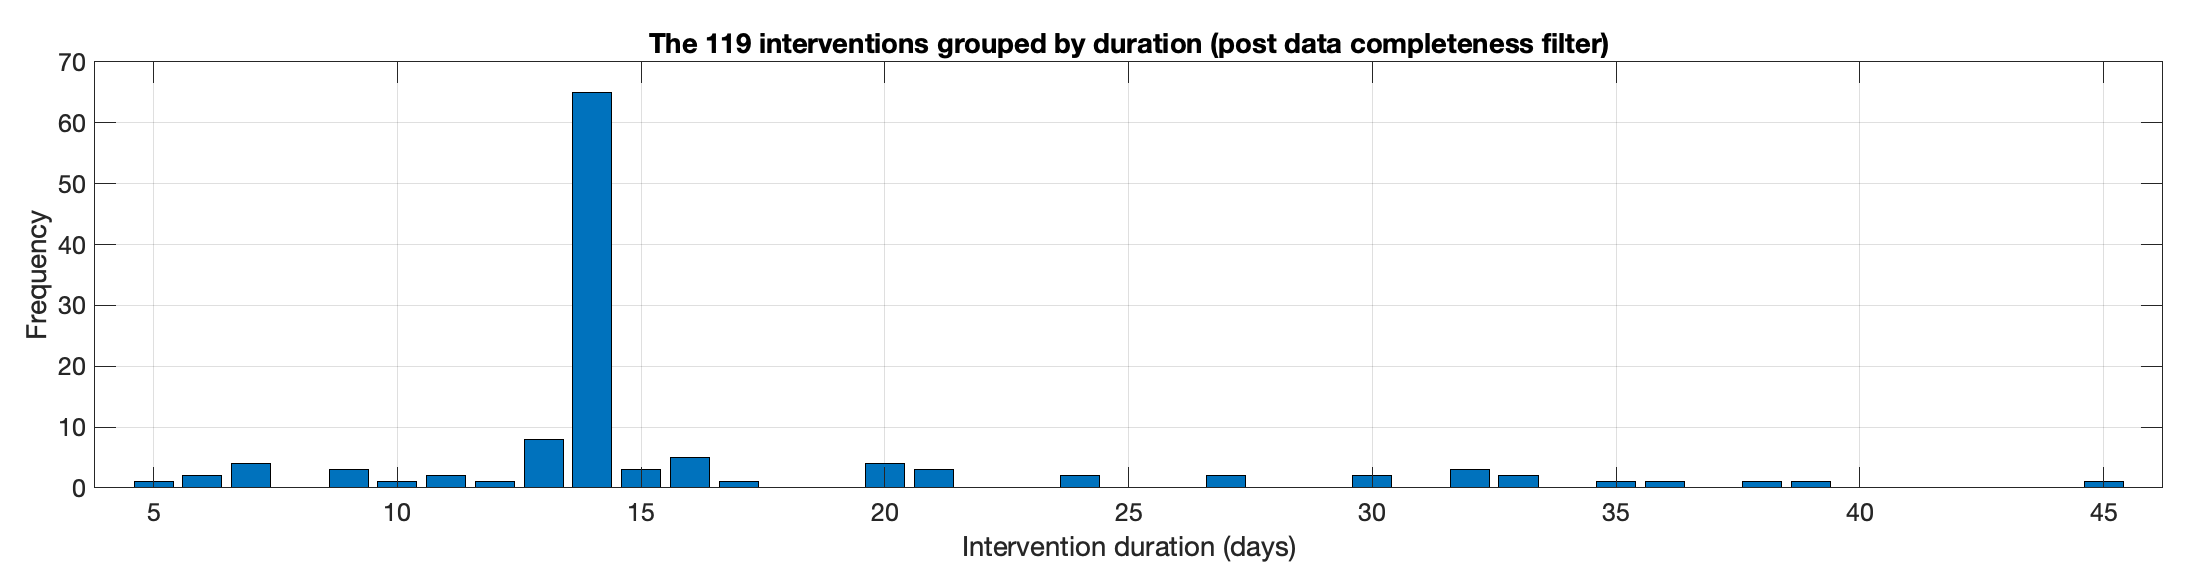
\includegraphics[width=150mm]{images/intrduration.png}
    \label{fig:intrbyduration}
    \end{figure}

    \item It should be small enough to have a sufficient amount interventions. Due to the scarcity of the data, the choice of D and the criteria for "insufficient data" stated in \ref{sec:intrlist} closely work together to define the amount of selected interventions, as shown in the table below.
    
    \vspace*{5px}
    \begin{center}
    \begin{tabular}{c|c} 
    \hline
        \textbf{D} & \textbf{Filtered interventions} \\
        \hline
        20 & 119 \\
        40 & 55 \\
    \hline
    \end{tabular} 
    \end{center}
    \vspace*{5px}
    
   This confirmed the choice for D = 20. 119 interventions is already a small sample size. In particular, the aim is to split the data in two or more folds, while learning different latent curves, a high amount of interventions is critical.

\end{itemize}

\subsection{Model dimensionality}
The number of bio-markers chosen is exactly the number of dimensions that will be studied by the model. The measures mask (mm) parameter filters a subset of M measures out the 18 listed in table \ref{tab:measures}. Note that \textit{measures} and \textit{bio-markers} from the biological vocabulary, and \textit{features} from the machine learning vocabulary are used as synonyms.

The rule of thumb to chose the model dimensionality is dual:
\begin{enumerate}
    \item Patients are a complex system whose behaviour is expected to be inferred using different types of features. This complexity can be met by increasing the data dimensionality. Unless bio-markers are extremely noisy and not correlated with the patient's status, they are kept. From thorough observation, calories, weight were removed because noisy and uncorrelated with events. Pusle rate was found to be more correlated to the recovery than resting heart rate. Minutes asleep and temperature seemed not correlated but were kept in doubt.
    \item Measures of the same family, e.g. "forced expiratory" based measures (FEV1, FEV6, FEF2575, etc) or subjective measures (wellness, cough), contain a similar patient information. Since each measure has the same weight in the calculation of the objective function, the model can be biased if one family is over-represented. To avoid point 2., only two measures from the FEV family were kept: FEV1 as a) it was the signal with clearest behaviour and b) it is the gold standard for respiratory measures in cystic fibrosis studies \cite{giron_2021}. FEF2575 was also used since a) during optimisation it showed increase model numerical stability and provided a lower objective function at end-state (average of 1.3 without and 1.27 with based on 13 runs), b) clinically it can provide more consistent signal than FEV1 for asymptomatic patients, whose number is subject to rise after the transition to the highly effective Trikafta CFTR modulator.
\end{enumerate}

Therefore cough, wellness, FEV1, FEF2575, pulse rate, O2 saturation, temperature, minutes asleep were selected, i.e. 8 dimensions.

A data density check was performed to avoid numerical instability on the typical profile. This could happen if there was a generalised absence of measurements at specific times from treatment accross all patients. Fore example during hospital intravenous antibiotics (IVs), the patient might be constrained by fatigue or equipment for some measurements (weight, spirometry). The heatmap of the measurements for all intervention on figure \ref{fig:heatmap} present an homogeneous at an intervention level and no specific patterns in the columns that could be expected.

\begin{figure}[!h]
    \caption{Heatmap of the amount of measurements recording (mm=34) for each intervention (line) and day in range [-25;39] around treatment start (1 pixel is one day)}
    \centering
    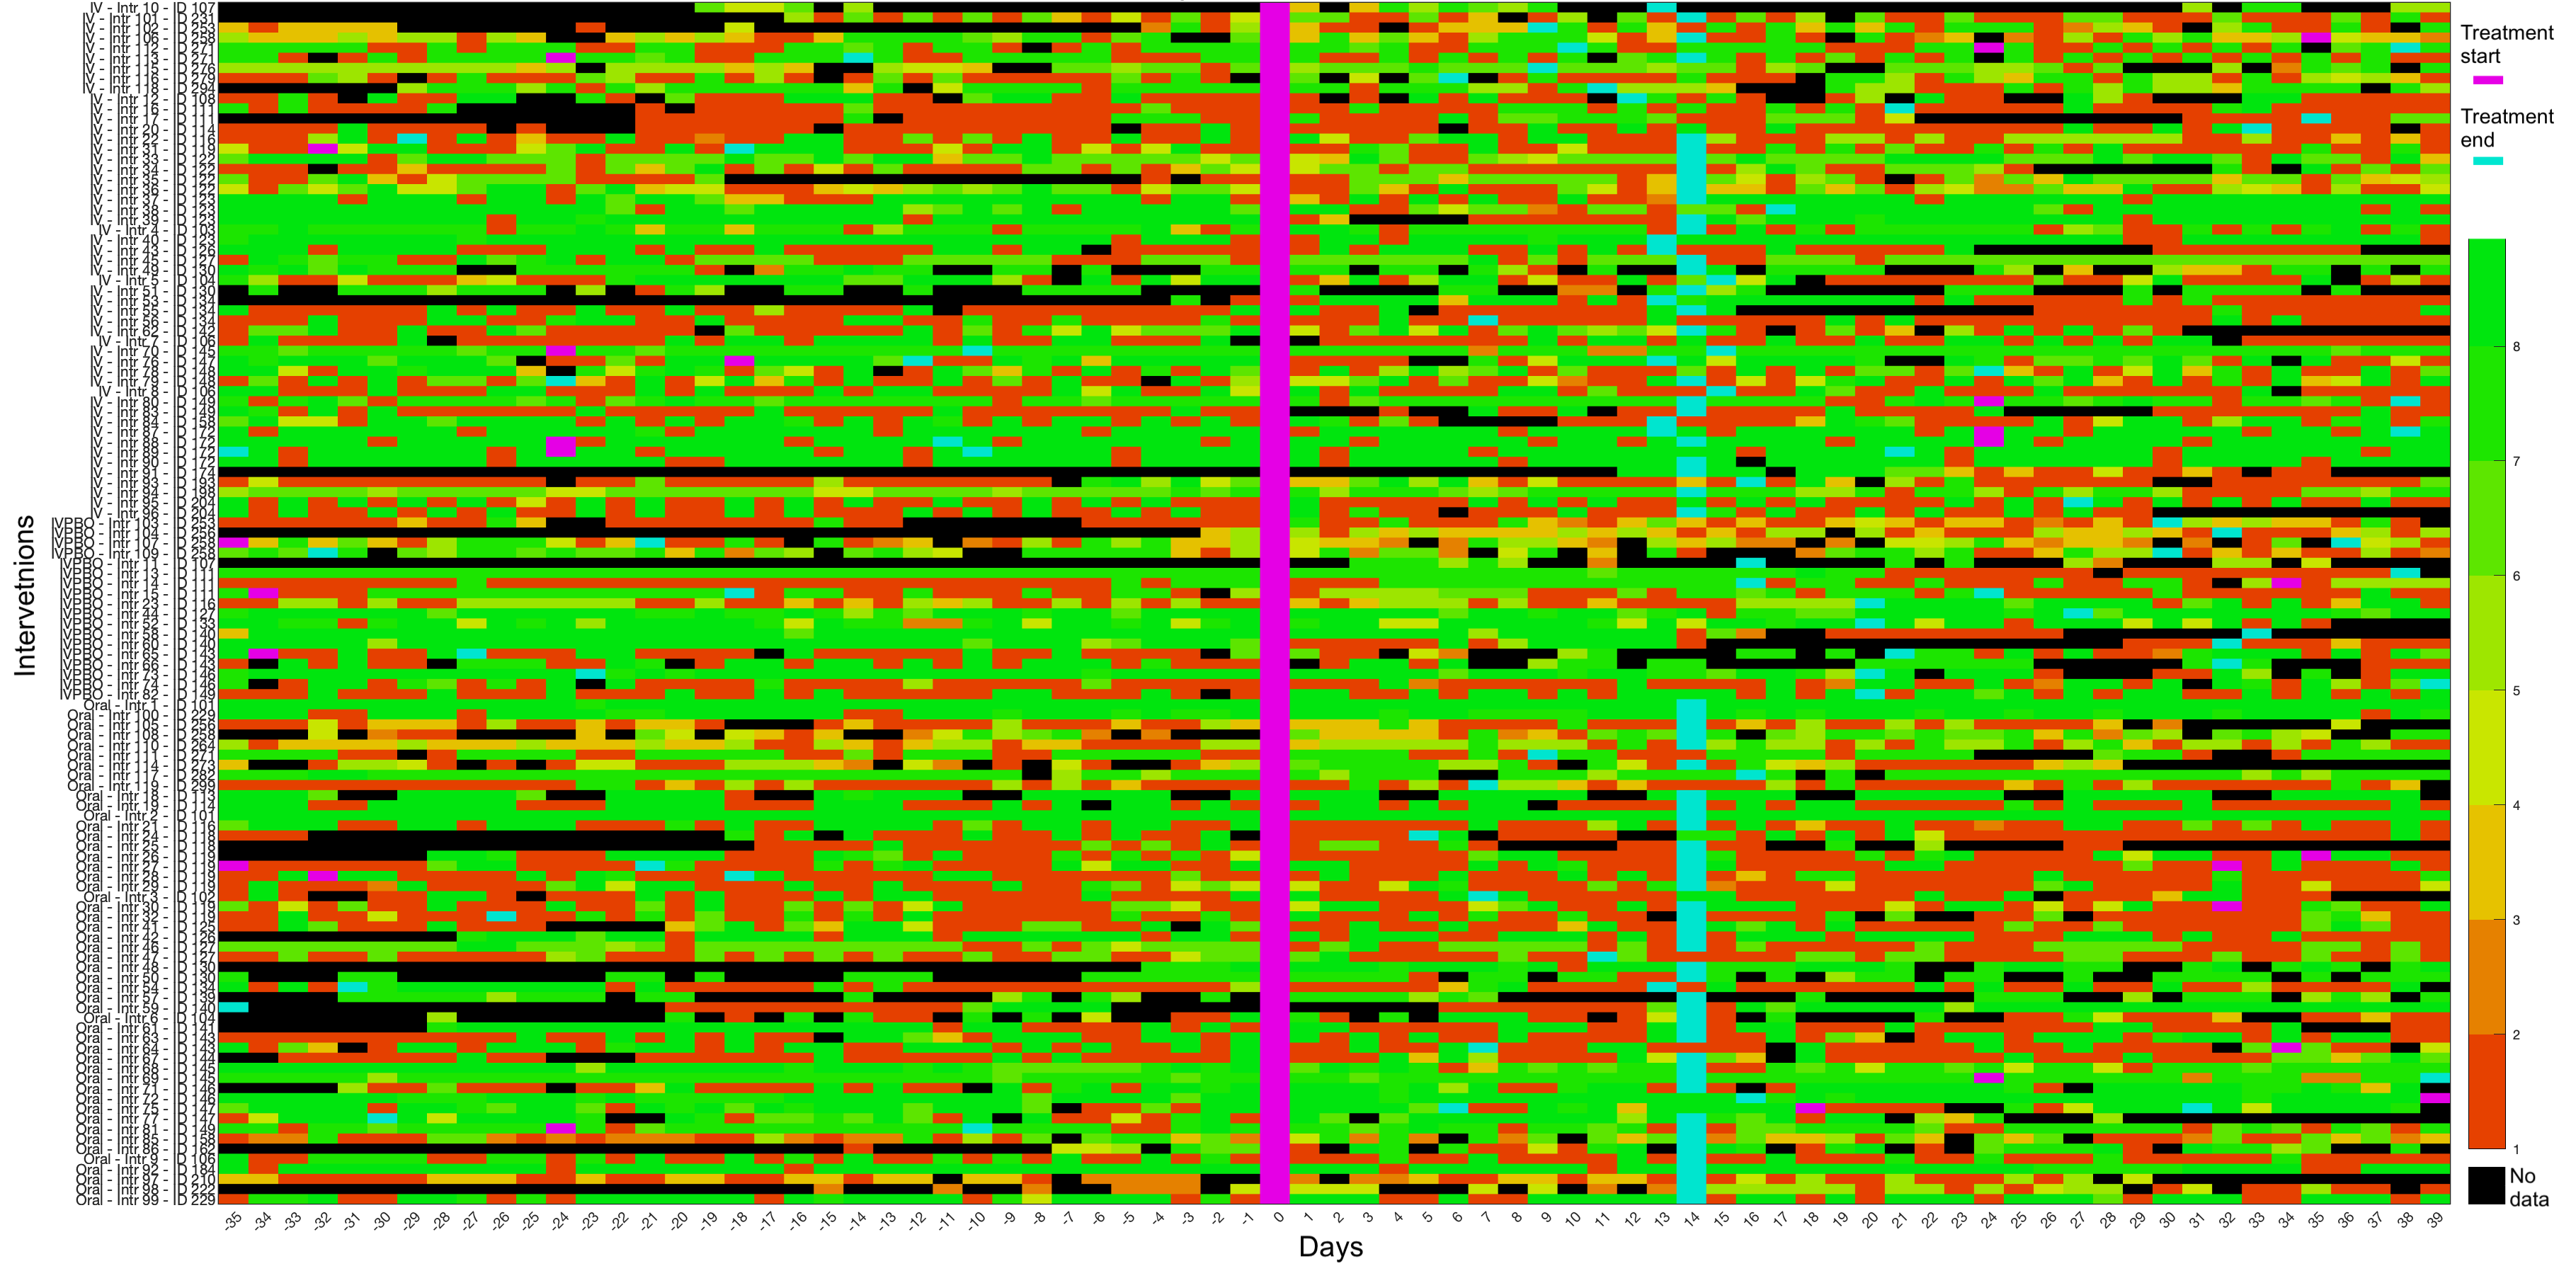
\includegraphics[width=150mm]{images/heatmapmm.png}
    \label{fig:heatmap}
\end{figure}

\subsection{Maximum offset}
The choice of this parameter is a trade-off between 1) minimising the objective function, 2) while having a sufficient point contribution for each day on the typical profile (chosen as at least 5 for one curve - referred to as \textit{count threshold}). For 1), the greater the offset the smaller the final objective function's value, see figure \ref{fig:offsets}. Issue 2) will arise on the left-most part, poor in data records contribution due to the right-shift without left-wise data imputation. The maximum offset was chosen by sequentially increasing its value and looking at the resulting typical profile, until the typical profile was imprecise on the left. mo > 16 lead to empty slots on the left-most part of the typical profile for FEV1 and wellness, see grey bar graph on figure \ref{fig:offsets}. FEV1 and wellness were chosen because they were representative of the other measures and subject to missing data (the median for the density of measurement over the whole study were respectively 19\% and 22\%, meaning 1.4 measurement per week). Therefore mo is set to 15.

\begin{figure}[!h]
    \caption{Maximum offset benchmark with inferred FEV1, wellness typical profiles for $mo \in \{10, 15, 16\}$ }
    \centering
    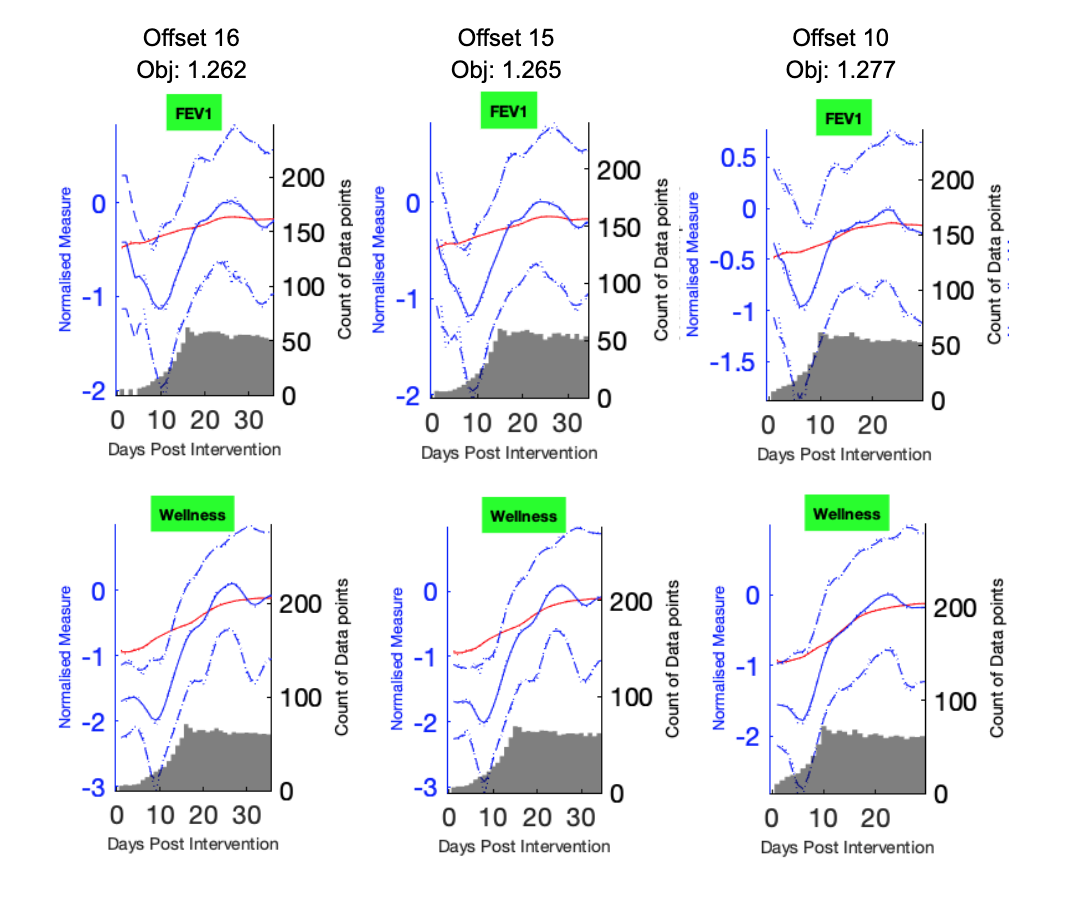
\includegraphics[width=90mm]{images/offsets1.png}
    \label{fig:offsets}
\end{figure} 
Note: on figure \ref{fig:offsets}, the blue curve is the typical profile (with mean in plain line and standard deviation in dotted line), the red curve indicates the unaligned profile, i.e. with all offsets forced to 0, and each grey bar in the bottom chart is the amount of data points contributing to the corresponding day on the typical profile.

\subsection{Maximum vertical shift}
The maximum vertical shift ($\alpha$ as defined and described in \ref{sec:vshift}) is fixed by running several models and comparing 1) the trend of the typical curve, 2) the distribution of vertical shift allocation. On the distributions, for the data records where the vertical shift is between the boundaries, the remaining vertical shift between the sample and the typical profile is fully cancelled. At the boundaries, the difference in mean is adjusted by $\alpha$ thus strengthening the importance of the underlying evolution in recovery over the difference in mean.
One can observe on figure \ref{fig:vshift} that the sensibility of  wellness (and also cough, minutes asleep, O2saturation, temperature) is low with respect to vertical shift. However, there is a minimum vertical shift of 0.4 necessary to allow to differentiate data records based on FEV1 (also generally all FEV measures and pulse rate). As two high values for this parameter cancel the difference of mean that can help differentiate two recoveries (\ref{sec:vshift}) $\alpha$ was set to 0.4 for the rest of the study. This is also the standard value used for the APE study \cite{damian}. Note that for two classes inference  $\alpha = 0.4$ is the value corresponding to the most robust model, see section \ref{sec:robustness}.

\begin{figure}[!h]
    \caption{Vertical shift benchmark with distribution and inferred FEV1, wellness typical profiles for $\alpha \in \{0, 0.2, 0.4, 0.7\}$ }
    \centering
    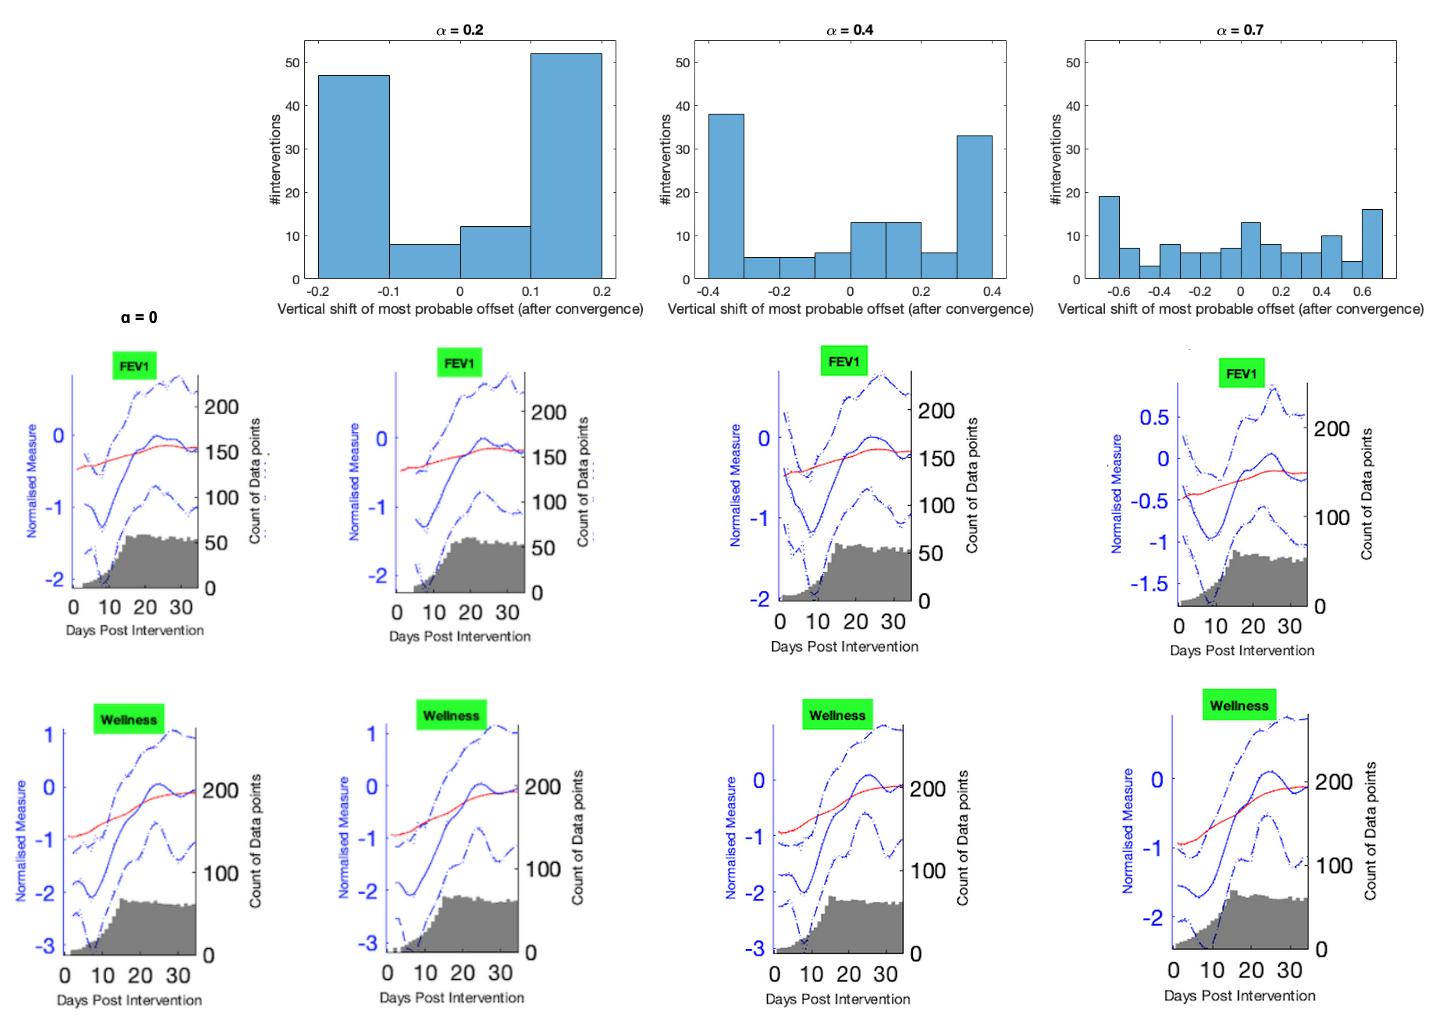
\includegraphics[width=140mm]{images/vshift.png}
    \label{fig:vshift}
\end{figure} 

\section{Generation of the typical recovery profile}
Given the chosen core parameters in \ref{sec:chosenparam}, the typical profile is drawn on figure \ref{fig:profile}. It is important to remember that the profile does not contain data prior to treatment start. 
\subsubsection{Graphical settings}
No vertical adjustment of the profiles were done. Therefore, the 0 on the y-axis corresponds to the stable baseline as defined in \ref{sec:normalisation}. The curves were smoothed with a 3 days window to filter day to day noise and improve the clarity of the final graph. Some left-most points are missing: there were not plotted because less than five data records' values contribute to them, i.e. there is too much uncertainty about their typical value. The typical curve for FEF2575 and temperature were not plotted because the first it had a very close behaviour to FEV1, and the latter did not seem to contain information related to the recovery.

\begin{figure}[!h]
    \caption{Typical profile derived with the probabilistic inference algorithm, with 119 data records}
    \centering
    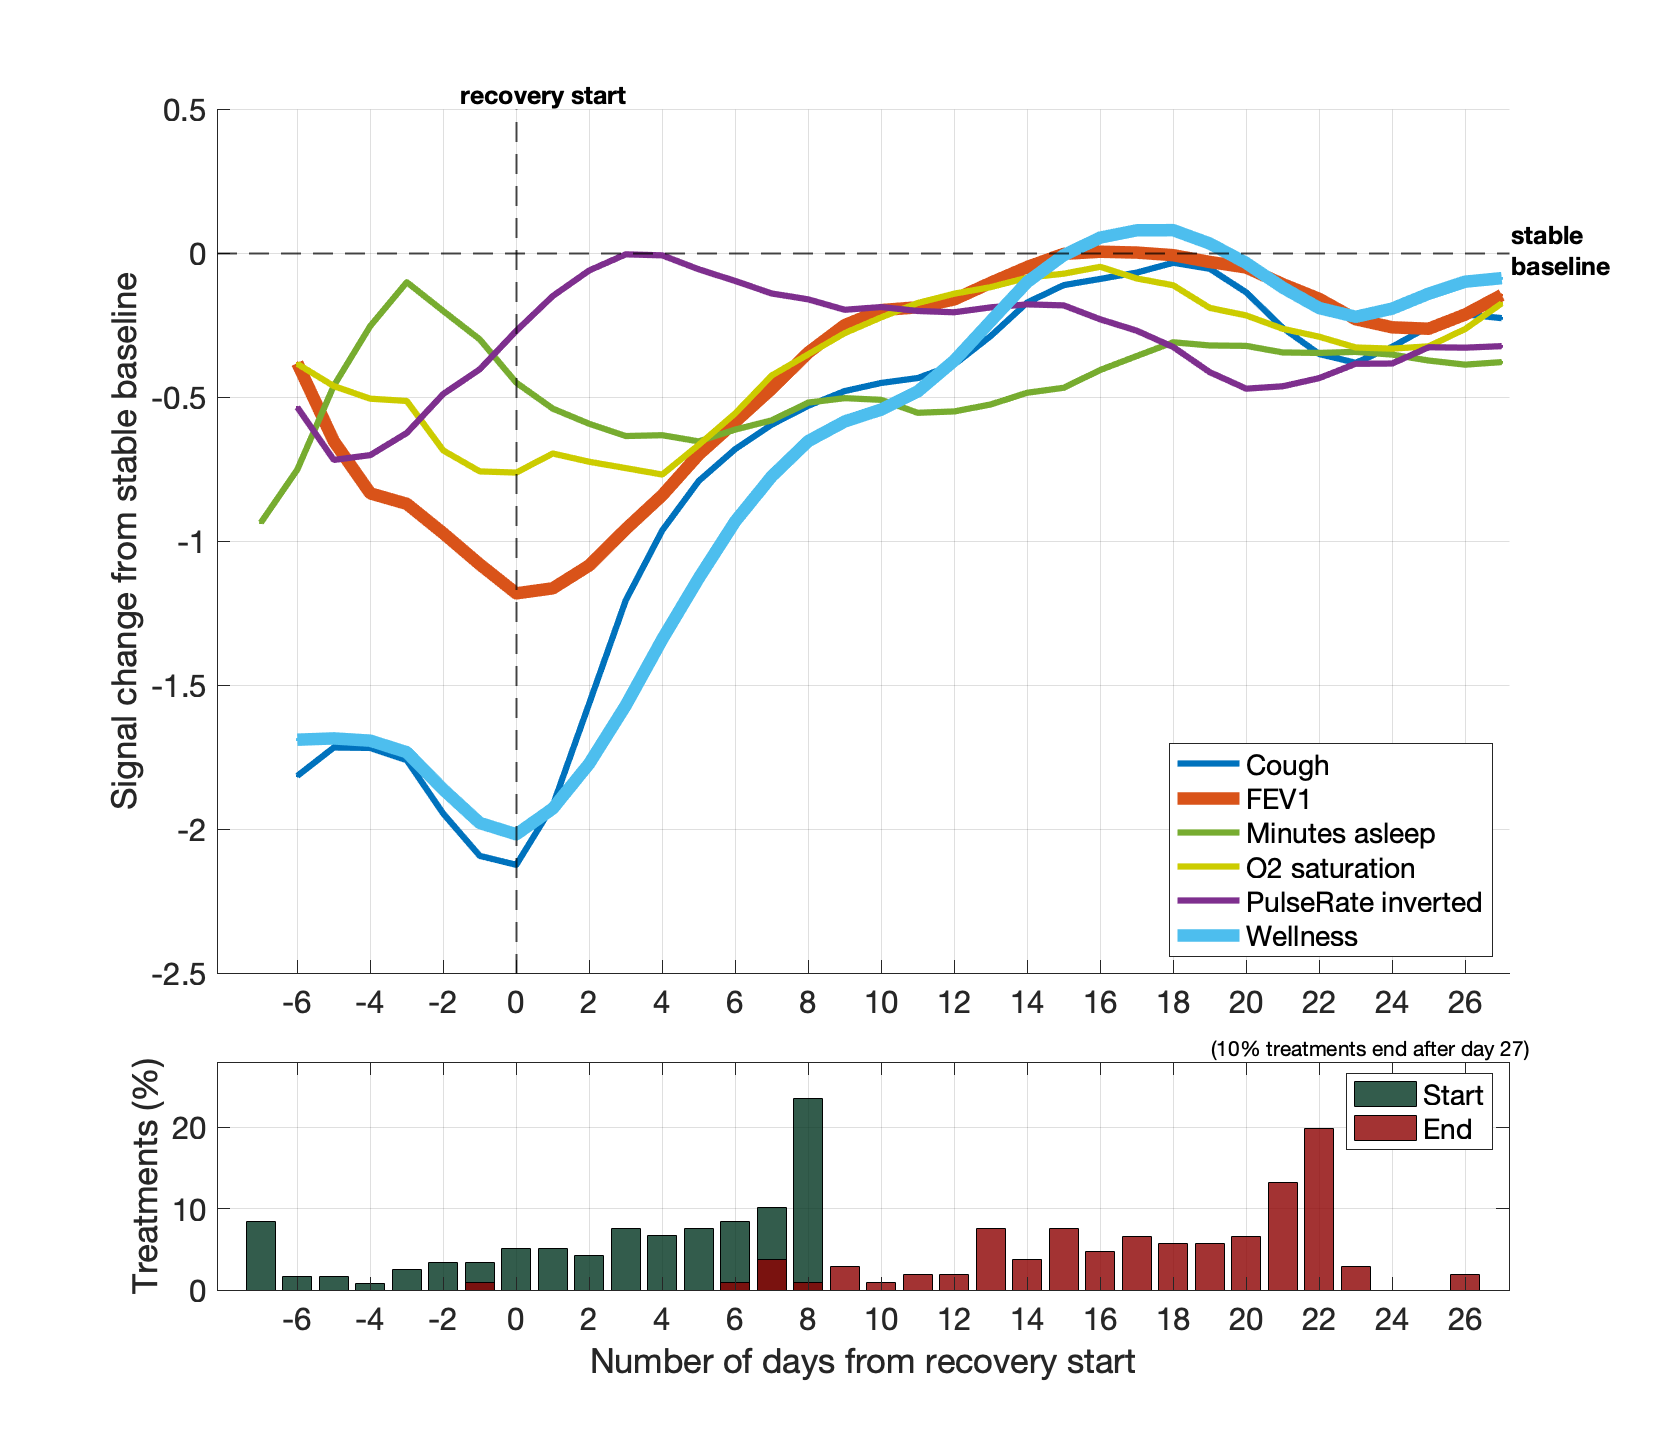
\includegraphics[width=100mm]{images/profile_typical.png}
    \label{fig:profile}
\end{figure}

\subsection{Terminology}
The terms used to analyse the recovery profiles are introduced here.

\textbf{Recovery start ($k_R$)} is defined to be the consensus beginning of increase for all measures. If unclear, a higher weight is given to FEV1 and wellness (highlighted with a thicker line on the graphs), which show the clearest contrast. At measures level, the recovery start is the beginning of increase for that measure. Any treatment starting after $k_R$ has a recovery start on the same day as the treatment start. Note that one can expect continuous decline that can sometimes be clinically explained by antibiotic resistance of the infection participating bacteria. In such cases, the recovery start is undefined.

\textbf{Time to (treatment) response ($\tau$)}: It is equal to the number of days between treatment start and recovery start. Based on our model, it can be computed for each intervention n with the offset $F_n$ and the recovery start $k_R$:
\begin{equation}
    \forall n \in N, \tau = 
    \begin{cases}
        k_R - F_n & \text{for } F_n < k_R\\
        0 & \text{for } F_n \geq k_R\\
    \end{cases}
\end{equation}
A time to treatment response of 0 means that the treatment had an effect on the signals within the day it was started.

%The values of the signals are in a
%\textbf{Recovery from partial decline:}  At treatment start, the signals are 

\textbf{Full recovery:} After treatment start, the signals come back to the stable baseline.

\textbf{Partial recovery:} After treatment start, the signals increase but do not come back to the stable baseline, i.e. the recovery is not full. This is an example of unsuccessful recovery.

\textbf{Successful recovery:} A recovery is defined as successful when the measures come back and stay "close" to the stable baseline. In literature, "close" is defined as 90\% of the stable baseline \cite{morgan_2017}.

The limit between \textbf{full decline} and \textbf{partial decline} is defined for reach signal at 25\% of the height between the lowest signal's point and the stable baseline. Looking at the typical profile, if most measures' profile contain values below the limit, the recovery starts from a full decline. Else, the recovery starts from a partial decline.

\subsection{Typical recovery profile observations}
The main concept behind the typical profile for recovery is that any D-day long physiological time-series immediately following a treatment can be placed on the matching measure of this profile with little error. Interventions that do not fit are considered as atypical with respect to this profile. This is reformulation of the model's first assumption defined in \ref{sec:datagen}. Looking at figure \ref{fig:profile}, one can note the following points:
\begin{itemize}
    \item FEV1, cough, wellness, O2 saturation have a closely similar behaviour with different amplitude.
    \item ~40\% of the recoveries start from a full decline, ~60\% from a partial decline, based on FEV1, cough and wellness.
    \item All patients' typically recover fully 14 days after the recovery start. There is a clear recovery climax 15-20 days after treatment start. After this, the signals undergo a call-back (slight decline) prior to their stabilisation.
    \item There is no sign of sharp decline after treatment end.
\end{itemize}

\subsection{Typical time to response}
The response to treatment $\tau$ is computed for all interventions on figure \ref{fig:tau}, based on the computed offsets and the determined recovery start. For over 90\% of the interventions, the response to treatment is 0, i.e. the recovery starts on the same day as treatment start. Note that the time to response can also be read on the bar graph of the treatment start, it is the gap in days between the treatment start and the recovery start.

\begin{figure}[!h]
    \caption{Typical time to response}
    \centering
    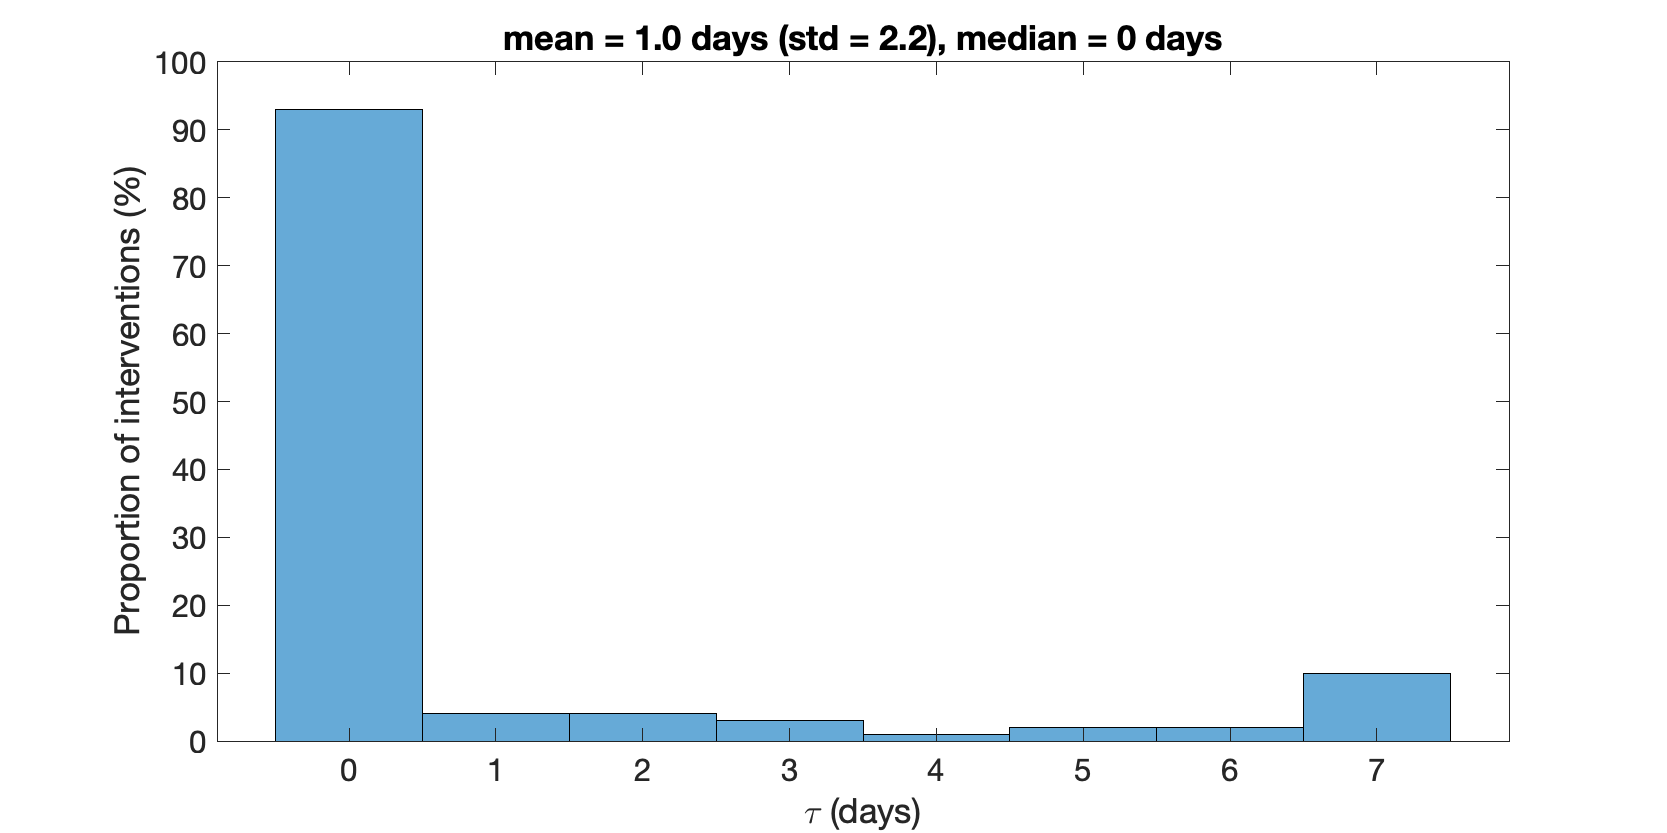
\includegraphics[width=90mm]{images/tautypical.png}
    \label{fig:tau}
\end{figure}

\section{Different types of recovery inference}
Now that the foundation of the typical profile was built, one would like to answer the question "Are there different types of recoveries?". The main interest is to create knowledge for the clinician. In this section, two types of recoveries are inferred and then mapped to patients' specificity, e.g. microbiology and lung volume. Additionally, the typical profile of an unsuccessful recovery is drawn.

\subsection{Model robustness}
The robustness against initialisation is the capacity of the model to provide the same end-states amid various initialisation-states. In the current settings, as all data records are randomly initialised to a class, and the end state is the mapping $\mathcal{F}$ described in \ref{sec:multiclass}. The robustness of the model was evaluated by initialising the model with different random seeds and comparing the end-states, for two latent curves.

\subsubsection{Class labels harmonisation with 2 latent curves}
Since the initialisation is random, the end-states are class-agnostic. In fact, the interventions corresponding to first class for one random seed can match the interventions corresponding to the second class of another random seed. Among the used random seeds, the set of interventions that had most in common with the class 1 of an end-state taken as reference were set to class 1 and the others were set to class 2.

\subsubsection{Model robustness for 2 latent curves} \label{sec:robustness}
The model was run 14 times with 7 different random seeds and 2 different maximum vertical shift, and a maximum iteration number of 120. When the maximum number of iterations was reached, results were taken as valid only if offset and latent curves had not changed since more than 5 iterations. Results for $\nu=0.4$ are given in table \ref{tab:nl2vs}. The random seed that minimised the objective function was taken as reference, e.g. rs1 for $\nu=0.4$. Figure \ref{fig:nl2classerror} shows the classification error for the corresponding end-state. An intervention with n errors was assigned \textit{n} times to the wrong class, and \textit{7-n} times to the right class. N=3 concerns outlying interventions, consistently switching between classes.

Relatively, $\nu=0.4$ is more optimal than $\nu=0.7$. Whereas $\nu=0.4$ provided 6 outlying interventions and over 80 interventions with 1-error or less, $\nu=0.7$ provided 19 outlying interventions and more 2-errors than 1-errors.

Globally with $\nu=0.4$, the model was considered as robust enough. In fact, for random seeds 1, 3, 5, 6, 7, a baseline of 72\% of interventions, were systematically belonging to the same class. The 5\% outlying interventions were also systematically the same, namely \{8; 41; 55; 94; 102; 104\}. Those outlying interventions did not show related characteristics, based on patient number, route, average measures per day, days with measures, offsets, and drug therapy. The resulting 23\% of interventions were switching between class 1 and class 2 depending on the initialisation state, highlighting slightly different relation between the features.

Hence, the model was consistent enough to infer two types of recoveries with $\nu=0.4$ and random seed 1, which provided the minimum the objective function.

\begin{figure}[!h]
    \caption{Classification error for $\nu$ = \{0.4; 0.7\}}
    \centering
    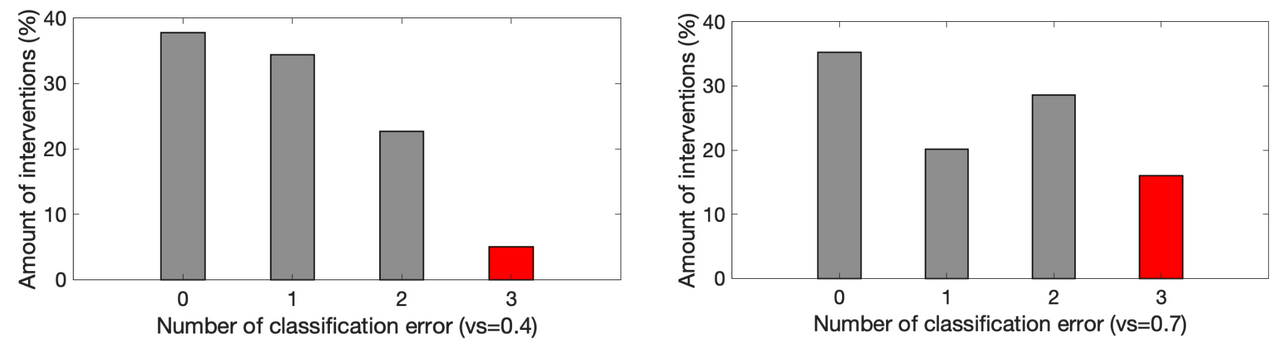
\includegraphics[width=100mm]{images/nl2classerror.png}
    \label{fig:nl2classerror}
\end{figure}

\begin{table}[!h]
    \centering
    \begin{tabular}{c|c|c|c|c|c|c}
        \hline
         \textbf{Random seed}& \textbf{Obj} & \textbf{Class 1} & \textbf{Class 2} & \textbf{ $\leq$ 1 error} & \textbf{3 errors} & \textbf{Iterations}\\
         \hline
         rs1 & 1.2243 & 63 & 56 & 72\% & 5\% & 120 \\
         rs2 & 1.2316 & 57 & 62 & 70\% & 5\% & 58 \\
         rs3 & 1.2313 & 43 & 76 & 72\% & 5\% & 120 \\
         rs4 & 1.2297 & 55 & 64 & 59\% & 21\% & 120 \\
         rs5 & 1.2283 & 42 & 77 & 72\% & 5\% & 91 \\
         rs6 & 1.2255 & 39 & 80 & 72\% & 5\% & 120 \\
         rs7 & 1.2306 & 39 & 80 & 72\% & 5\% & 120 \\
         \hline
    \end{tabular}
    \caption{Model run results for 7 different initialisation-states, $\nu=0.4$}
    \label{tab:nl2vs}
\end{table}

%Through each iteration, the algorithm then allocates the samples (data records) to the current best matching unit (latent curve). After convergence, the end-state is the mapping $\mathcal{F}$ described in \ref{sec:model}. 

%The inferred classes with n latent curves are a n-fold partition of the 119 data records. 

\subsection{Two distinct typical recoveries}
The model was run to infer two distinct classes of recoveries. Given the model's robustness analysis, the core parameters and graphical settings were chosen identically to the ones for the typical profile.

The class 1, figure \ref{fig:profileC1C2}, show interventions with partial recoveries. ~77\% of recoveries start from a full decline (days [-11; 2]). The time to response is highly left-skewed with a maximum of 11 days. There is a similar call back to the one on the typical profile.

The class 2, figure \ref{fig:profileC1C2}, show very different behaviour. Wellness, cough and FEV1 show a full recovery at day 9, therefore much earlier than on the typical profile, that goes beyond the stable baseline and far higher than on the typical profile. One can note that pulse rate does not show to be related to the recovery. ~43\% of recoveries start from a full decline (days [-6; 2]). The time to response is left-skewed with a maximum of 6 days.

\begin{figure}[!h]
    \caption{Class 1 profile with 53\% of data records (left), Class 2 profile with 47\% of data records (right)}
    \centering
    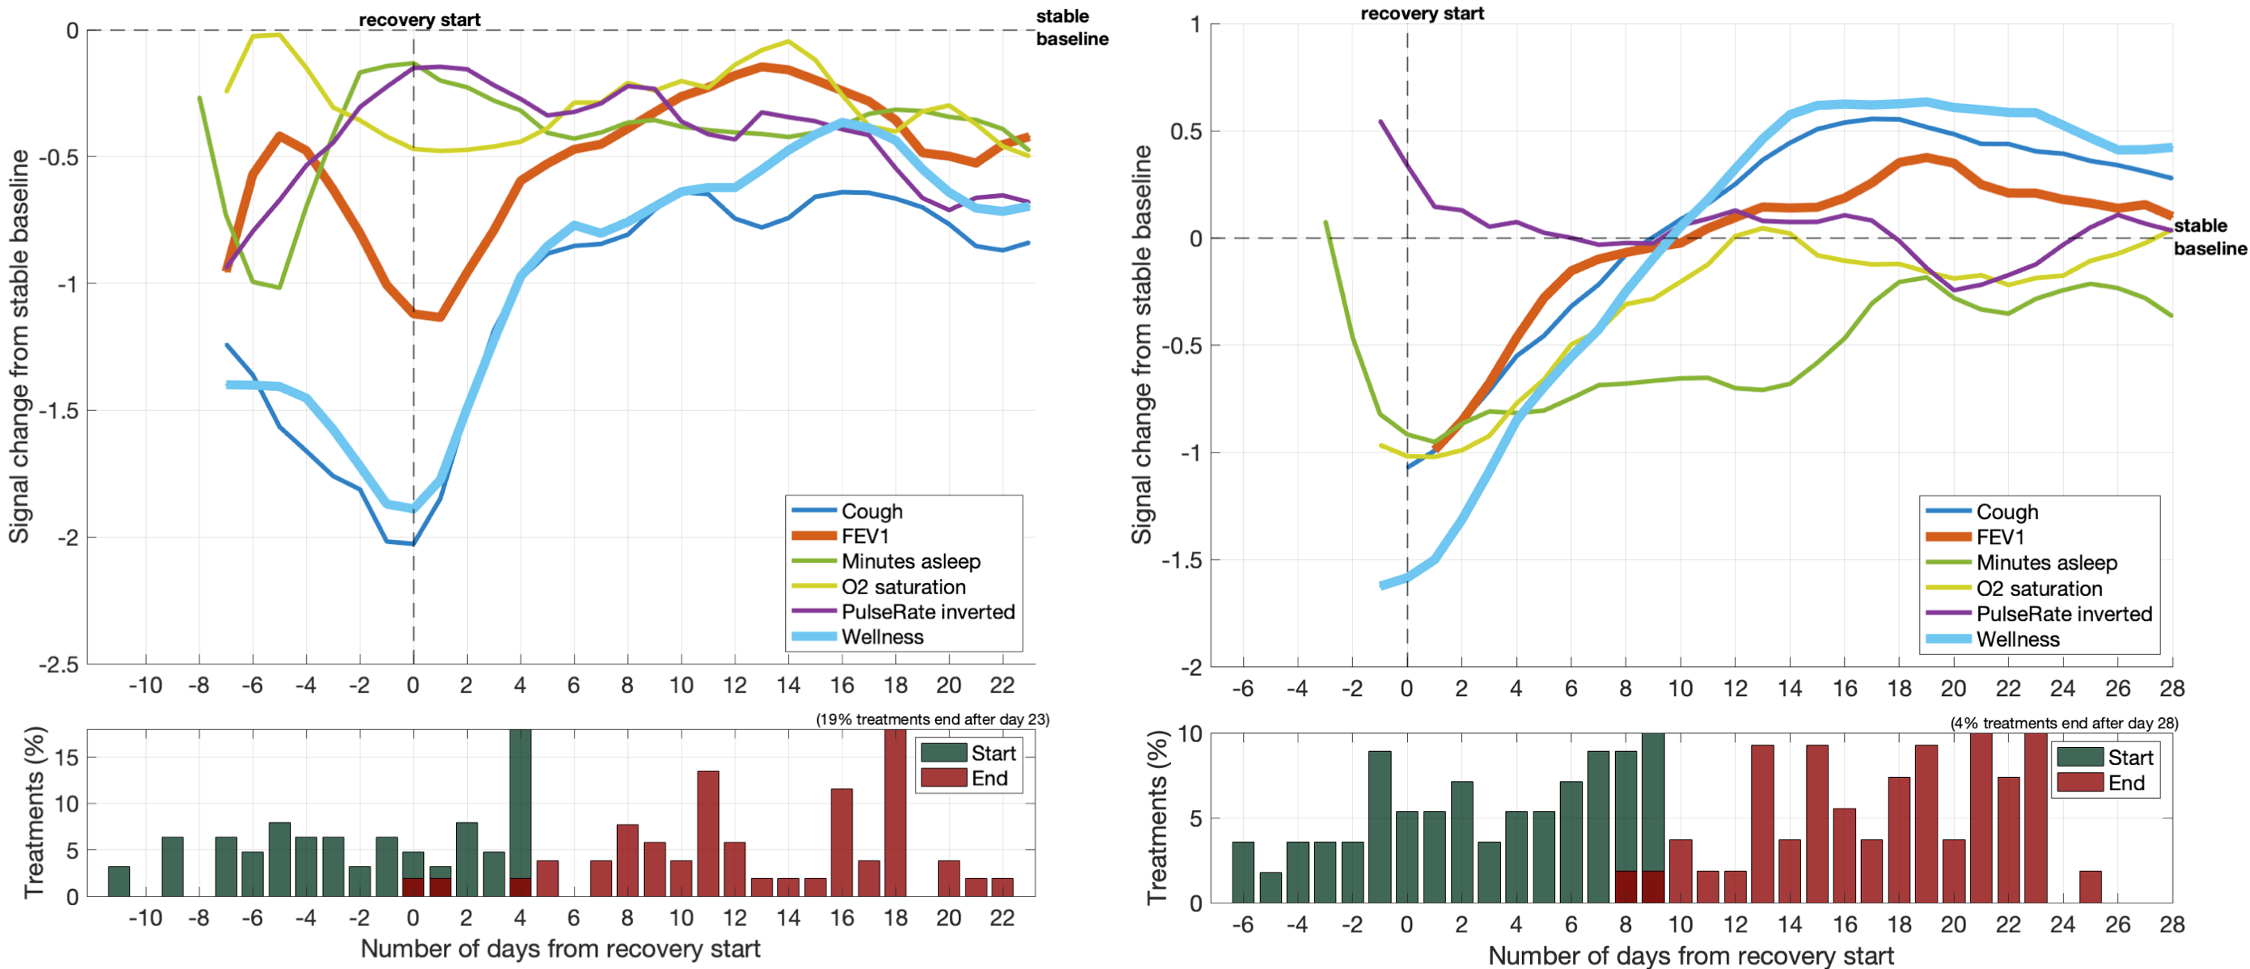
\includegraphics[width=160mm]{images/nl2.png}
    \label{fig:profileC1C2}
\end{figure}

\subsection{Relation with patients characteristics}
Relation between patients' characteristics and classes were computed through hypothesis testing, after removing the 6 outlying interventions. Wilcoxon signed-rank test was used to test the null hypothesis that data in Class 1 and Class 2 are samples from continuous distributions with equal medians. Chi-Square Goodness-of-Fit test was used to test the null hypothesis that the data in Class 1 fits the distribution of the data in Class 2. This was used for binary data, e.g. sex, presence of an infection, as the distributions need not be continuous. A significance level of 0.01 was chosen to limit the amount of type II errors. 

In the results of the hypothesis tests summarised in figure \ref{fig:pvalue}, Class 2 recoveries are more commonly found in people with a high number of antibiotic treatments and in particular IV treatments over the study period. Note that class 1 and class 2 contained IV or Oral treatment in balanced proportion, roughly half-half. People with chronic pseudomonas aeruginosa infections more likely to experience recoveries of Class 2. 

    \begin{figure}[!h]
    \caption{Hypothesis tests results, for $\alpha=0.01$}
    \centering
    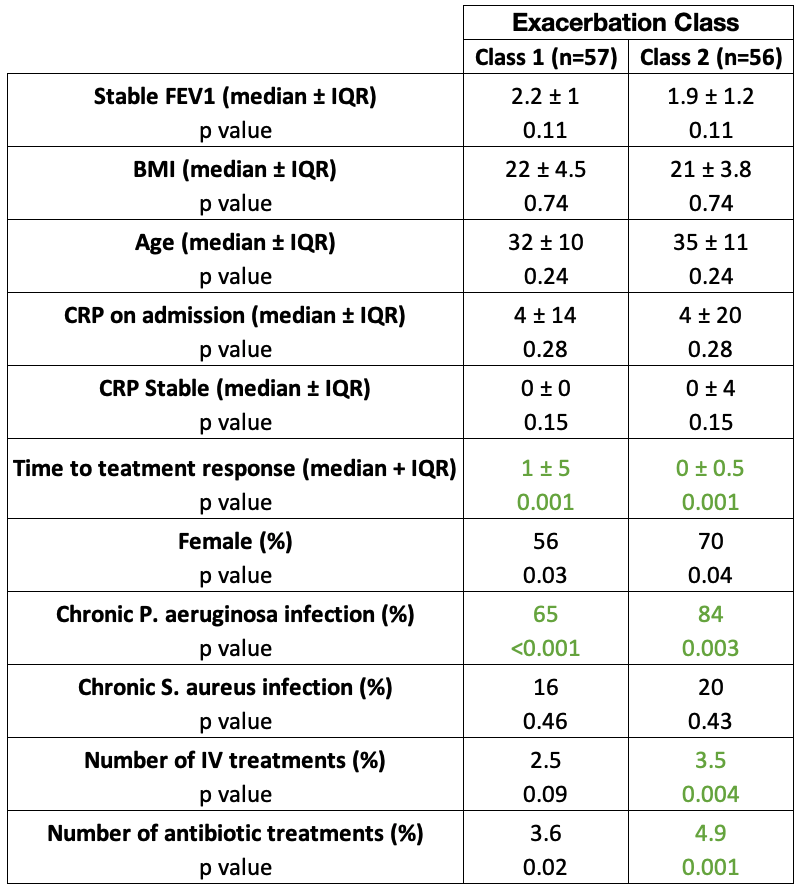
\includegraphics[width=70mm]{images/pvalue.png}
    \label{fig:pvalue}
    \end{figure}

\subsection{Typical profile of a full recovery with decline}
The previous analyses did not present clear signs of a special type of unsuccessful recovery where the signals undergo a full or almost-full recovery swiftly followed by a clear decline. Clinically, this is commonly known in the case of repeated APEs, where the patient degrades again right after treatment. One could wondered whether the model can also be used to characterise this type of recovery.

While observing the data records, 35 cases showed a decline before or after the end of the treatment. A model was run with this subset of interventions. On figure \ref{fig:fail}, most signals including FEV1 undergo a slight increase from day -2 to day 12 up to the stable baseline, followed by a decrease of same amplitude from day 12 to day 32. Note that the consensus decline start on day 20 happens when ~40\% of treatments are not finished. Cough and wellness are the only measures with a clear increase as a response to treatment. Also, ~25\% of treatments start after day 8 of this profile, and are characterised by an absence of response to treatment. 

\begin{figure}[!h]
    \caption{Typical profile of a recovery with decline (30\% of interventions)}
    \centering
    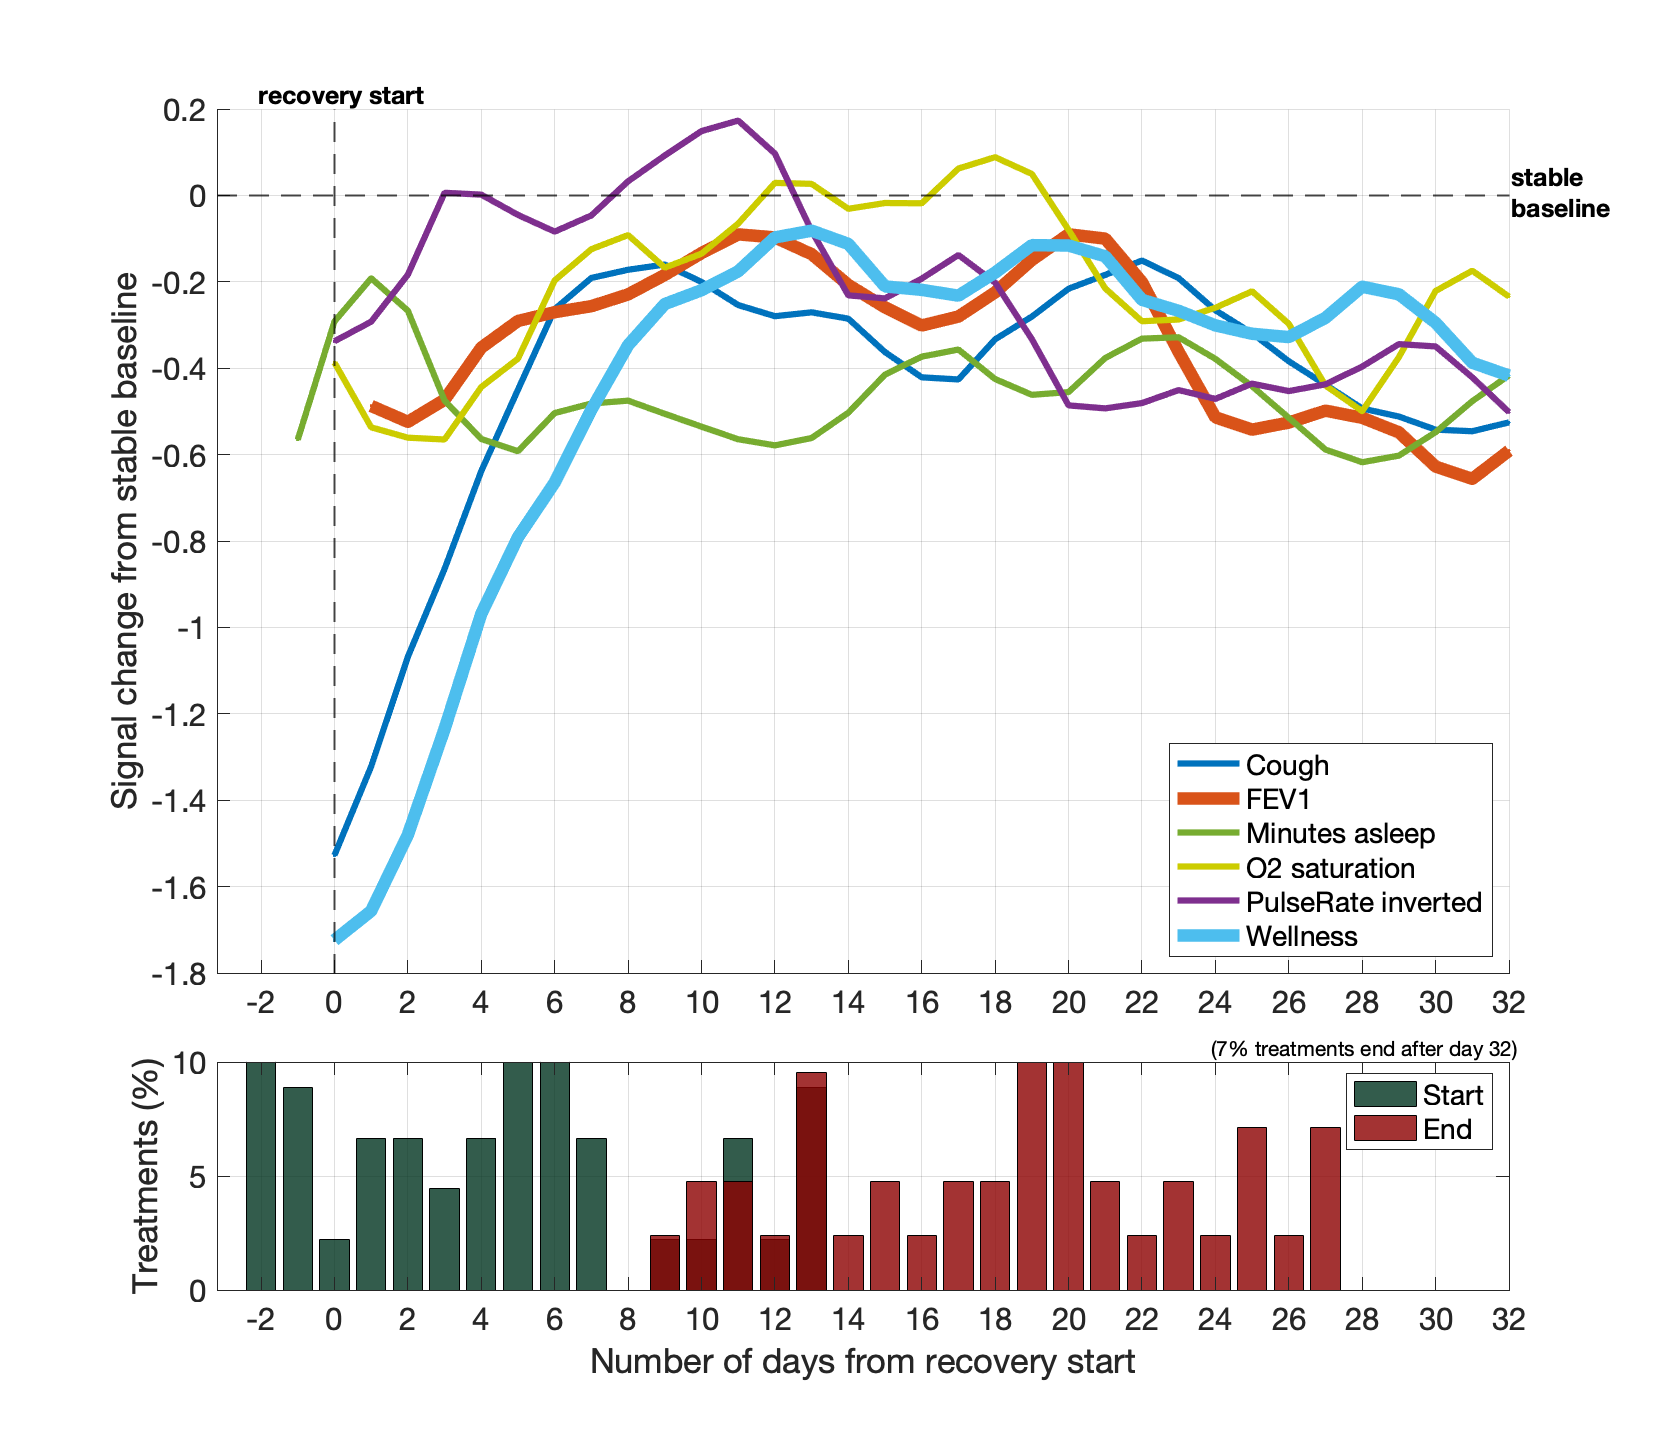
\includegraphics[width=100mm]{images/profile_fail.png}
    \label{fig:fail}
\end{figure}

\section{Recovery definition}
Thanks to the previous results and observation, a recovery can be defined as as follows: 

\definition A recovery is a process of change in the patient's health status following an antibiotic treatment, closely linked to the preceding acute pulmonary exacerbation. It lasts from the treatment start until the day where a recovery label can be assigned with sufficient certitude. A recovery can be analysed through the observation of different sets of physiological bio-markers. Elective treatments are defined as treatments that seemed not preceded by an APE.

The recovery label can be set according to the process on figure \ref{fig:types}. Example for a label: "unsuccessful partial recovery from full decline".

\begin{figure}[!h]
    \caption{Directed graph that can be used to label recoveries}
    \centering
    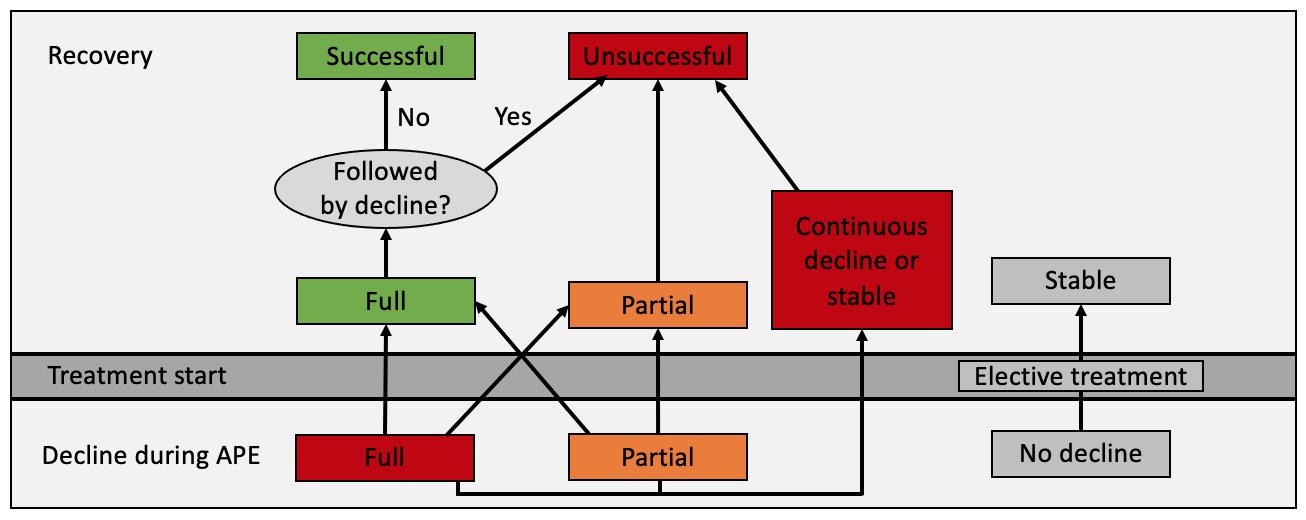
\includegraphics[width=130mm]{images/types.png}
    \label{fig:types}
\end{figure}



%\section{Slope based classification of a recovery}
%Based on our analysis, 
%When we asked ourselves the question "What is a recovery from antibiotics?", it appeared that there was no clear classification nor definition of the different types of recoveries. Clinicians can easily list the different types of recoveries from antibiotic treatments based on their multi patient experience, but we are unsure if there nuances or consensus in the clinician community. We suggest that during each clinics following an antibiotic treatment, recoveries could be labelled according to this classification. Similar longitudinal evolution of the recovery labels could help group patients together and treat them according

%From a clinical perspective, we can expect different types of intervention summarized in the following table:
%Literature well defines everything linked to a recovery, but not the recoveries themselves. Classifiation of 